\section{Hierarchization on Dimensionally Adaptive Sparse Grids}
\label{sec:43dimAdaptive}

\minitoc{77mm}{7}

\noindent
Dimensionally adaptive sparse grids,
which are sums of different hierarchical subspaces
as described in \cref{sec:232dimensionallyAdaptiveSG},
have the advantage over general spatially adaptive sparse grids
that algorithms can be formulated and applied more easily.
In this section, we describe two methods:
first, the well-known combination technique, which was
already mentioned in \cref{sec:232dimensionallyAdaptiveSG},
and second, a new algorithm based on residual interpolation.



\subsection{The Combination Technique and Its Combinatorial Proof}
\label{sec:431combiTechniqueProof}

The combination technique was one of the first methods that
were developed by Griebel et al. in \cite{Griebel92Combination}
(for two and three dimensions)
after the term ``sparse grids'' was coined in 1991 \cite{Zenger91Sparse}.
However, the combination technique predates the development of sparse grids
by decades, as it was already mentioned by Smolyak in 1963
\multicite{Smolyak63Quadrature,Hegland07Combination}.
Delvos developed and proved the standard combination formula in the
framework of Boolean interpolation operators in 1982
\multicite{Delvos82Dvariate,Delvos89Boolean}.

\paragraph{Formal description and outline of a combinatorial proof}

In the following, we give a formal description of the
sparse grid combination technique, and we outline a new combinatorial proof
of its correctness.
While we discuss a high-level explanation of the proofs in this section,
the proofs themselves can be found in \cref{sec:a131proofCombiTechnique},
since most of them are rather technical.
For simplicity,
we formulate the combination technique and its proof for regular
sparse grids (see \cref{sec:231regularSG}).
However, the main ideas of the chain of proofs are also applicable
to dimensionally adaptive sparse grids
(see \cref{sec:232dimensionallyAdaptiveSG}).

\begin{theorem}[sparse grid combination technique]
  \label{thm:combiTechnique}
  Let $\liset \ceq \{(\*l, \*i) \mid
  \normone{\*l} \le n,\; \*i \in \hiset{\*l}\}$
  correspond to the regular sparse grid
  $\regsgset{n}{d}$ and let $(\fcnval{\*l,\*i})_{(\*l,\*i) \in \liset}$
  be given function values on $\regsgset{n}{d}$.
  If we define
  \begin{itemize}
    \item
    the combined sparse grid interpolant $\regsgintp[\ct]{n}{d}$ via
    \eqref{eq:combiTechnique}, i.e.,
    \begin{equation}
      \regsgintp[\ct]{n}{d}
      = \sum_{q=0}^{d-1} (-1)^q \binom{d-1}{q} \sum_{\normone{\*l'} = n-q}
      \fgintp{\*l'},
    \end{equation}
    where $\fgintp{\*l'} \in \ns{\*l'}$ is the full grid interpolant
    of $\objfun$ with level $\*l'$, and
    
    \item
    the hierarchical sparse grid interpolant $\regsgintp{n}{d}$
    via \eqref{eq:hierarchizationProblem} and
    \eqref{eq:hierarchizationInterpolant}
  \end{itemize}
  and if we assume that the hierarchical splitting equation
  \eqref{eq:hierSplittingMV} holds,
  then the combined and the hierarchical sparse grid interpolants coincide:
  \begin{equation}
    \regsgintp[\ct]{n}{d}
    = \regsgintp{n}{d}.
  \end{equation}
\end{theorem}

\begin{proof}[Proof (sketch)]
  Let $\gp{\*l,\*i} \in \regsgset{n}{d}$ be an arbitrary
  point of the regular sparse grid.
  First, we split the inner sum of $\regsgintp[\ct]{n}{d}(\gp{\*l,\*i})$
  into levels $\*l'$ whose full grid sets $\fgset{\*l'}$
  contain $\gp{\*l,\*i}$ and levels whose full grid sets
  do not contain $\gp{\*l,\*i}$:
  \begin{equation}
    \regsgintp[\ct]{n}{d}(\gp{\*l,\*i})
    = \sum_{q=0}^{d-1} (-1)^q \binom{d-1}{q} \cdot \paren*{
      \sum_{\substack{\normone{\*l'} = n - q\\\fgset{\*l'} \ni \gp{\*l,\*i}}}
      \fgintp{\*l'}(\gp{\*l,\*i}) +
      \sum_{\substack{\normone{\*l'} = n - q\\\fgset{\*l'} \notni \gp{\*l,\*i}}}
      \fgintp{\*l'}(\gp{\*l,\*i})
    }.
  \end{equation}
  The summands $\fgintp{\*l'}(\gp{\*l,\*i})$ of the first inner sum
  each equal $\fcnval{\*l,\*i}$ due to the full grid interpolation
  property \eqref{eq:interpFullGridMV}.
  Therefore, the first inner sum is equal to the product of
  $\fcnval{\*l,\*i}$ with the number of summands:
  \begin{equation}
    \label{eq:combiTechniqueSplitSum}
    \begin{split}
      \regsgintp[\ct]{n}{d}(\gp{\*l,\*i})
      &= \fcnval{\*l,\*i} \cdot \sum_{q=0}^{d-1} (-1)^q \binom{d-1}{q} \cdot
      \setsize{
        \{\*l' \mid \normone{\*l'} = n - q,\; \fgset{\*l'} \ni \gp{\*l,\*i}\}
      }\\
      &\qquad{} {} + \sum_{q=0}^{d-1} (-1)^q \binom{d-1}{q} \cdot
      \sum_{\substack{\normone{\*l'} = n - q\\\fgset{\*l'} \notni \gp{\*l,\*i}}}
      \fgintp{\*l'}(\gp{\*l,\*i}).
    \end{split}
  \end{equation}
  After this sketch of proof,
  we will prove that the first of the two summands in
  \cref{eq:combiTechniqueSplitSum}
  equals one (see \cref{prop:combiTechniqueOne})
  and that the second of the two summands
  equals zero (see \cref{prop:combiTechniqueZero}).
  Consequently, we infer
  \begin{equation}
    \regsgintp[\ct]{n}{d}(\gp{\*l,\*i})
    = \fcnval{\*l,\*i},
  \end{equation}
  i.e., $\regsgintp[\ct]{n}{d}$ interpolates $\objfun$ at $\regsgset{n}{d}$.
  Note that $\regsgintp[\ct]{n}{d}$ is contained in $\regsgspace{n}{d}$,
  if the hierarchical splitting equation \eqref{eq:hierSplittingMV} holds,
  as
  \begin{equation}
    \fgintp{\*l'} \in
    \ns{\*l'}
    = \bigoplus_{\*l''=\*0}^{\*l'} \hs{\*l''}
    \subset \regsgspace{n}{d},\quad
    \normone{\*l'} \le n,
  \end{equation}
  due to $\normone{\*l''} \le \normone{\*l'} \le n$
  for $\*l'' \le \*l'$, i.e.,
  $\hs{\*l''} \subset \regsgspace{n}{d}$ for
  $\*l'' = \*0, \dotsc, \*l'$.%
  \footnote{%
    This argumentation can be straightforwardly adapted
    for general dimensionally adaptive sparse grids
    with downward closed level sets as mentioned in
    \cref{sec:232dimensionallyAdaptiveSG}.%
  }
  As both $\regsgintp[\ct]{n}{d}$ and $\regsgintp{n}{d}$
  are contained in $\regsgspace{n}{d}$ and
  interpolate $\objfun$ on $\regsgset{n}{d}$, they coincide
  due to the uniqueness of sparse grid interpolation
  (linear independence of the hierarchical basis).
\end{proof}

\paragraph{Inclusion-exclusion principle}

It remains to prove that the first sum in \eqref{eq:combiTechniqueSplitSum}
is indeed one and that the second sum vanishes.
The first statement is a direct consequence of the
\term{inclusion-exclusion principle} \cite{Hegland07Combination}.
In its simplest form, the idea of the principle is that the cardinality
of the union of two finite subsets $A$ and $B$ of some set is given by
\begin{equation}
  \setsize{A \cup B}
  = \setsize{A} + \setsize{B} - \setsize{A \cap B},
\end{equation}
i.e., we first count (include)
the elements in $A$ and then in $B$,
but as we have counted the elements of $A \cap B$ twice,
we have to subtract (exclude) its cardinality again.

The setting is similar for the combination technique.
If we add all grids in \cref{fig:combinationTechnique}
on the green diagonal, then every point whose index is not odd
will be counted multiple times.
By subtracting the number of occurrences of the points on the
red diagonal,
the result of the ``weighted counting'' is exactly one for every point.
The following proposition, whose proof is of purely combinatorial nature,
generalizes this argument to higher dimensions:

\begin{restatable}[inclusion-exclusion principle]{%
  proposition%
}{%
  propCombiTechniqueOne%
}
  \label{prop:combiTechniqueOne}
  For every $\gp{\*l,\*i} \in \regsgset{n}{d}$, we have
  \begin{equation}
    \label{eq:combiTechniqueOne}
    \sum_{q=0}^{d-1} (-1)^q \binom{d-1}{q} \cdot
    \setsize{
      \{\*l' \mid \normone{\*l'} = n - q,\; \fgset{\*l'} \ni \gp{\*l,\*i}\}
    }
    = 1.
  \end{equation}
\end{restatable}

\begin{proof}
  See \cref{sec:a131proofCombiTechnique}.
\end{proof}

\paragraph{Canceling out function values}

The second statement about the vanishing second sum in
\eqref{eq:combiTechniqueSplitSum} is much harder to prove.
It says that at every grid point $\gp{\*l,\*i}$,
the contributions $\fgintp{\*l'}$ of levels $\*l'$
that do not contain that point cancel out,
which may seem quite surprising.
The key observation is as follows:
The values of $\fgintp{\*l'}, \fgintp{\*l''}$ for two levels
$\*l', \*l''$ are the same at $\gp{\*l,\*i}$,
if all non-equal entries $l'_t, l''_t$ of the levels are
each greater or equal to $l_t$.

For a higher-level explanation,
note that the statement $l'_t \ge l_t$ is equivalent to
$\fgset{l'_t} \ni \gp{l_t,i_t}$.
Both $\fgintp{\*l'}, \fgintp{\*l''}$ interpolate at
$\gp{\*l,\*i}$ when projected onto the $t$-th dimension,
so their contribution to $\fgintp{\*l'}(\gp{\*l,\*i})$ and
$\fgintp{\*l''}(\gp{\*l,\*i})$ must be the same.
Although there may be dimensions $t$ for which
$\fgset{l'_t} \notni \gp{l_t,i_t}$,
these dimensions do not matter if $l'_t = l''_t$,
as the univariate restrictions of $\fgintp{\*l'}, \fgintp{\*l''}$
interpolate the same data, and they are evaluated at the same point
$\gp{l_t,i_t}$.

One can formalize these considerations by defining an
equivalence relation on the set of levels such that the values of
$\fgintp{\*l'}$ at $\gp{\*l,\*i}$ are constant
on the equivalence classes.

\begin{definition}[%
  equivalence relation for the proof of the combination technique%
]
  \label{def:combiTechniqueEquivalenceRelation}
  Let $\gp{\*l,\*i} \in \regsgset{n}{d}$ be fixed and
  \begin{equation}
    \label{eq:combiTechniqueSpecialLevelSet}
    L
    \ceq \{\*l' \mid \ex{q=0,\dotsc,d-1}{
      \normone{\*l'} = n - q,\; \fgset{\*l'} \notni \gp{\*l,\*i}
    }\}
  \end{equation}
  be the set of levels that do not contain $\gp{\*l,\*i}$.
  We define a relation $\eq$ on $L$ as follows:
  For $\*l', \*l'' \in L$, we set $\*l' \eq \*l''$ if and only if
  \begin{equation}
    \falarge{t \notin T_{\*l',\*l''}}{\min\{l'_t, l''_t\} \ge l_t},\quad
    T_{\*l',\*l''}
    \ceq \{t \mid l'_t = l''_t < l_t\}.
  \end{equation}
\end{definition}

\begin{restatable}[identical values in equivalence classes]{%
  shortlemma%
}{%
  lemmaCombiTechniqueIdenticalValues%
}
  \label{lemma:combiTechniqueIdenticalValues}
  Let $\*l', \*l'' \in L$ with $\*l' \eq \*l''$.
  Then, $\fgintp{\*l'}(\gp{\*l,\*i})
  = \fgintp{\*l''}(\gp{\*l,\*i})$.
\end{restatable}

\begin{proof}
  See \cref{sec:a131proofCombiTechnique}.
\end{proof}

By exploiting the tensor product structure of the basis functions,
the proof shows an even stronger version, which is shown
in \cref{fig:combiTechniqueProof}:
The components $\fgintp{\*l'}$ and $\fgintp{\*l''}$ are equal
on the $m$-dimensional affine subspace through $\gp{\*l,\*i}$
parallel to the $m$ coordinates in $T_{\*l',\*l''}$
(where $m \ceq \setsize{T_{\*l',\*l''}}$).
The lemma allows us to group summands in the second sum of
\eqref{eq:combiTechniqueSplitSum} by function values.
Hence, it remains to count the number of levels in
each equivalence class of $\eq$.
Therefore, we need a characterization of the equivalence classes:

\begin{SCfigure}
  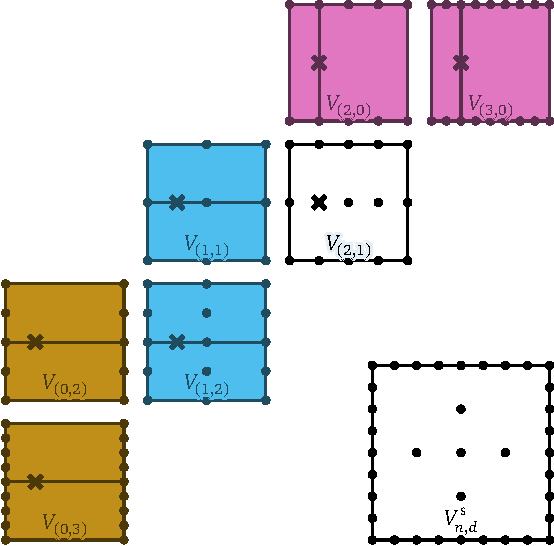
\includegraphics{combiTechniqueProof_1}%
  \caption[%
    Canceling out function values in the proof of the combination technique%
  ]{%
    Nodal subspaces $\ns{\*l}$ contributing to the combination
    technique solution for the two-dimensional regular sparse grid
    $\regsgspace{n}{d}$ of level $n = 3$ \emph{(bottom right).}
    After picking a point $\gp{\*l,\*i} \in \regsgset{n}{d}$
    (\emph{cross,} here $\*l = (2, 1)$, $\*i = (1, 1)$),
    the set $L$ of levels whose grids do not contain $\gp{\*l,\*i}$
    \emph{(colored subspaces)}
    decompose into three disjoint equivalence classes
    \emph{(colors)} given by the relation $\eq$.
    In every equivalence class $L_0 \in \eqclasses{L}{\eq}$,
    the interpolants $\fgintp{\*l'}$ ($\*l' \in L_0$)
    equal on an affine subspace
    \emph{(dark lines),} which contains $\gp{\*l,\*i}$.
    Due to the combination coefficients,
    the contribution to the combined solution
    vanishes per equivalence class.%
  }%
  \label{fig:combiTechniqueProof}%
\end{SCfigure}

\begin{restatable}[characterization of equivalence classes]{%
  lemma%
}{%
  lemmaCombiTechniqueCharacterization%
}
  \label{lemma:combiTechniqueCharacterization}
  Let $L_0 \in \eqclasses{L}{\eq}$ be an equivalence class of $\eq$.
  If we define
  \begin{equation}
    T_{L_0}
    \ceq \{t \mid \exfa{l^\ast_t < l_t}{\*l' \in L_0}{l'_t = l^\ast_t}\}
  \end{equation}
  as the set of dimensions $t$ in which all levels in $L_0$
  have the same entry $l^\ast_t < l_t$, then
  \begin{equation}
    L_0
    = \{\*l' \in L \mid
    \fa{t \in T_{L_0}}{l'_t = l^\ast_t},\;
    \fa{t \notin T_{L_0}}{l'_t \ge l_t}\}.
  \end{equation}
\end{restatable}

\begin{proof}
  See \cref{sec:a131proofCombiTechnique}.
\end{proof}

The lemma states that every equivalence class $L_0$ is exactly the
set of the levels whose entries are equal
and smaller than $l_t$ in some dimensions
(which are contained in $T_{L_0}$)
and whose entries are greater or equal than $l_t$ in all other dimensions.
While this statement may seem intuitively correct,
the proof is rather technical.
Finally, we are now able to show that the second sum in
\eqref{eq:combiTechniqueSplitSum} vanishes:

\begin{restatable}[function value cancellation]{%
  proposition%
}{%
  propCombiTechniqueZero%
}
  \label{prop:combiTechniqueZero}
  For every $\gp{\*l,\*i} \in \regsgset{n}{d}$, we have
  \begin{equation}
    \sum_{q=0}^{d-1} (-1)^q \binom{d-1}{q} \cdot
    \sum_{\substack{\normone{\*l'} = n - q\\\fgset{\*l'} \notni \gp{\*l,\*i}}}
    \fgintp{\*l'}(\gp{\*l,\*i})
    = 0.
  \end{equation}
\end{restatable}

\begin{proof}
  See \cref{sec:a131proofCombiTechnique}.
\end{proof}

The proof essentially first counts the number of possible levels in
an equivalence class and then applies known combinatorial identities
to prove that the sum must vanish.
This proves \thmref{thm:combiTechnique}.



\subsection{Hierarchization with the Combination Technique}
\label{sec:432hierarchizationCombiTechnique}

It is straightforward to hierarchize function values
$\fcnval{\*l,\*i}$ on dimensionally adaptive sparse grids
with the combination technique.
The resulting hierarchization algorithm is given as \cref{alg:combiTechnique}.
In \cref{line:algCombiTechnique1},
the hierarchical surpluses corresponding to the full grid
interpolant $\fgintp{\*l'} \in \ns{\*l'}$ have to be computed
(see \eqref{eq:interpFullGridMV}).
As shown in \cref{sec:42fullGrids}, we can easily calculate these
surpluses with the unidirectional principle in
\cref{alg:unidirectionalPrinciple}.
The surpluses are then combined with the same combination formula
as in \thmref{thm:combiTechnique}.
Note that it is imperative to employ the hierarchical basis functions
$\basis{\*l,\*i}$ with $\*l = \*0, \dotsc, \*l'$ and $\*i \in I_{\*l}$
and not the nodal basis,
i.e., $\basis{\*l',\*i'}$ with $\*i' = \*0, \dotsc, \*2^{\*l'}$.

\begin{algorithm}
  \begin{algorithmic}[1]
    \Function{$\vlinout = \texttt{combinationTechnique}$}{%
      $\vlinin$, $n$, $d$%
    }
      \For{$q = 0, \dotsc, d - 1$}
        \For{$\*l' \in \natz^d$ with $\normone{\*l'} = n - q$}
          \State{%
            Let $(\surplus[(\*l')]{\*l,\*i})_{
              \*l = \*0, \dotsc, \*l'\!,\, \*i \in \hiset{\*l}
            }$ be such that
            $\sum_{\*l=\*0}^{\*l'} \sum_{\*i \in \hiset{\*l}}
            \surplus[(\*l')]{\*l,\*i} \basis{\*l,\*i} \equiv
            \fgintp{\*l'}$%
          }
          \label{line:algCombiTechnique1}
          \State{%
            $\surplus[(\*l')]{\*l,\*i} \gets 0$
            for all $(\*l,\*i) \in \liset$
            with $\lnot(\*l \le \*l')$%
          }
          \Comment{extend surpluses}%
          \label{line:algCombiTechnique2}
        \EndFor{}
      \EndFor{}
      \State{%
        $\linout{\*l,\*i}
        = \sum_{q=0}^{d-1} (-1)^q \binom{d-1}{q}
        \sum_{\normone{\*l'} = n-q} \surplus[(\*l')]{\*l,\*i}$
        for all $(\*l, \*i) \in \liset$%
      }
      \Comment{combine surpluses}%
    \EndFunction{}
  \end{algorithmic}
  \caption[%
    Hierarchization with the combination technique%
  ]{%
    Application of the hierarchization operator $\linop = \intpmatinv$
    with the combination technique.
    For simplicity,
    the algorithm is described for regular sparse grids,
    but it can be generalized to arbitrary dimensionally adaptive sparse grids.
    Inputs are
    the vector $\vlinin = (\linin{\*l,\*i})_{(\*l,\*i) \in \liset}$
    of input data (function values $\fcnval{\*l,\*i}$ at the grid points),
    the level $n$, and the dimensionality $d$ of the regular sparse grid,
    where $\liset$ is the set of all feasible level-index pairs $(\*l,\*i)$,
    i.e., $\normone{\*l} \le n$, $\*i \in \hiset{\*l}$.
    The output is the vector
    $\vlinout = (\linout{\*l,\*i})_{(\*l,\*i) \in \liset}$
    of output data (hierarchical surpluses $\surplus{\*l,\*i}$).%
  }%
  \label{alg:combiTechnique}%
\end{algorithm}

\paragraph{Correctness}

Of course, the proof of the correctness of \cref{alg:combiTechnique}
relies on the correctness of the combination technique
(see \cref{thm:combiTechnique}).
If determining the combination coefficients correctly
\cite{Nobile16Adaptive}, the algorithm can even be applied to
all dimensionally adaptive sparse grids.
The proof of the following proposition can be generalized accordingly.

\begin{proposition}[correctness of combination technique]
  \label{prop:correctnessAlgCombiTechnique}
  \Cref{alg:combiTechnique}
  is correct for hierarchization on regular sparse grids.
\end{proposition}

\begin{proof}
  According to \cref{line:algCombiTechnique1} of \cref{alg:combiTechnique},
  the full grid interpolants $\fgintp{\*l'}$ can be written as
  \begin{equation}
    \fgintp{\*l'}
    = \sum_{\normone{\*l} \le n} \sum_{\*i \in \hiset{\*l}}
    \surplus[(\*l')]{\*l,\*i} \basis{\*l,\*i}
  \end{equation}
  where the surpluses have been extended
  from $\*l = \*0, \dotsc, \*l'$ to all $\*l$ with $\normone{\*l} \le n$
  by zero in \cref{line:algCombiTechnique2}.
  \Cref{thm:combiTechnique} now allows to write the hierarchical
  interpolant $\regsgintp{n}{d}$ in terms of the full grid components:
  \begin{subequations}
    \begin{align}
      \regsgintp{n}{d}
      = \regsgintp[\ct]{n}{d}
      &= \sum_{q=0}^{d-1} (-1)^q \binom{d-1}{q} \sum_{\normone{\*l'} = n-q}
      \fgintp{\*l'}\\
      &= \sum_{q=0}^{d-1} (-1)^q \binom{d-1}{q} \sum_{\normone{\*l'} = n-q}
      \sum_{\normone{\*l} \le n} \sum_{\*i \in \hiset{\*l}}
      \surplus[(\*l')]{\*l,\*i} \basis{\*l,\*i}.\\
      \label{eq:propCorrectnessAlgCombiTechnique1}
      &= \sum_{\normone{\*l} \le n} \sum_{\*i \in \hiset{\*l}}
      \underbrace{
        \paren*{
          \sum_{q=0}^{d-1} (-1)^q \binom{d-1}{q} \sum_{\normone{\*l'} = n-q}
          \surplus[(\*l')]{\*l,\*i}
        }
      }_{= \linout{\*l,\*i}}
      \basis{\*l,\*i},
    \end{align}
  \end{subequations}
  where $\linout{\*l,\*i}$ is the $(\*l,\*i)$-th entry of the output vector
  of \cref{alg:combiTechnique}.
  Note that the hierarchical interpolant $\regsgintp{n}{d}$
  can be written as
  $\regsgintp{n}{d} = \sum_{\normone{\*l} \le n} \sum_{\*i \in \hiset{\*l}}
  \surplus{\*l,\*i} \basis{\*l,\*i}$
  (see \eqref{eq:regularSGInterpolant}),
  where the surpluses $\surplus{\*l,\*i}$ are unique due to the
  linear independence of the hierarchical basis.
  As \eqref{eq:propCorrectnessAlgCombiTechnique1}
  equals $\regsgintp{n}{d}$ and has the same form,
  the coefficients $\linout{\*l,\*i}$
  must coincide with the surpluses $\surplus{\*l,\*i}$.
\end{proof}



\subsection{Hierarchization with Residual Interpolation}
\label{sec:433residualInterpolation}

Another method to hierarchize function values on
dimensionally adaptive sparse grids is the
\term{method of residual interpolation.}
The advantage over the combination technique is that
it only needs to operate on so-called \term{active nodal spaces.}
In contrast, the combination technique needs to perform computations
on additional non-active nodal subspaces
(for the regular sparse grid case:
summands with $q \ge 1$ in \eqref{eq:combiTechnique}).

\paragraph{Active nodal spaces}

\Cref{alg:residualInterpolation} describes the procedure of
the method of residual interpolation,
given the function values $\vlinin$ corresponding to the grid points
and the levels $L$ contained in the sparse grid
(see \eqref{eq:dimensionallyAdaptiveSG}).
The list $\*l^{(1)}, \dotsc, \*l^{(m)}$ of active nodal spaces
in \cref{line:algResidualInterpolation1} is determined by the condition
\begin{equation}
  \label{eq:activeNodalSpaces}
  \bigcup_{j=1}^m \{\*l \in \natz^d \mid \*l \le \*l^{(j)}\} = L,\quad
  \falarge{j_1 \not= j_2}{\lnot(\*l^{(j_1)} \le \*l^{(j_2)})}.
\end{equation}
This means that the corresponding sparse grid $\sgset$
is the (non-disjoint) union of the full grid sets $\fgset{\*l^{(j)}}$
($j = 1, \dotsc, m$)
and no full grid set is contained in another, i.e.,
no full grid set can be omitted without
removing points from the union $\sgset$.

\begin{algorithm}
  \begin{algorithmic}[1]
    \Function{$\vlinout = \texttt{residualInterpolation}$}{%
      $\vlinin$, $\levelset$%
    }
      \State{%
        $r^{(0)}(\gp{\*l,\*i}) \gets \fcnval{\*l,\*i}$
        for all $(\*l,\*i) \in \liset$%
      }
      \State{%
        Compute list $\*l^{(1)}, \dotsc, \*l^{(m)}$
        of active nodal spaces from $L$ (see \eqref{eq:activeNodalSpaces})%
      }
      \label{line:algResidualInterpolation1}
      \State{%
        Sort $\*l^{(1)}, \dotsc, \*l^{(m)}$ by decreasing level sum%
      }
      \For{$j = 1, \dotsc, m$}
        \State{%
          Let $r_{\*l^{(j)}}^{(j-1)} \in \ns{\*l^{(j)}}$ be the
          interpolant of $r^{(j-1)}$ on $\fgset{\*l^{(j)}}$%
        }
        \label{line:algResidualInterpolation3}
        \State{%
          Let $(\surplus[(j)]{\*l,\*i})_{(\*l,\*i) \in \liset}$ be such that
          $\sum_{\*l=\*0}^{\*l^{(j)}} \sum_{\*i \in \hiset{\*l}}
          \surplus[(j)]{\*l,\*i} \basis{\*l,\*i}
          \equiv r_{\*l^{(j)}}^{(j-1)}$%
        }
        \Comment{interpolation}%
        \label{line:algResidualInterpolation2}
        \State{%
          $r^{(j)}(\gp{\*l,\*i}) \gets
          r^{(j-1)}(\gp{\*l,\*i}) - r_{\*l^{(j)}}^{(j-1)}(\gp{\*l,\*i})$
          for all $(\*l,\*i) \in \liset$%
        }
        \Comment{new residuals}%
        \label{line:algResidualInterpolation4}
      \EndFor{}
      \State{%
        $\vlinout \gets \sum_{j=1}^{m} \vsurplus^{(j)}$
        (where $\surplus[(j)]{\*l,\*i} = 0$,
        $(\*l,\*i) \in \liset$,
        if $\lnot(\*l \le \*l^{(j)})$)%
      }
      \Comment{combine surpluses}%
    \EndFunction{}
  \end{algorithmic}
  \caption[%
    Hierarchization with residual interpolation%
  ]{%
    Application of the hierarchization operator $\linop = \intpmatinv$
    with residual interpolation
    for dimensionally adaptive sparse grids.
    Inputs are
    the vector $\vlinin = (\linin{\*l,\*i})_{(\*l,\*i) \in \liset}$
    of input data (function values $\fcnval{\*l,\*i}$ at the grid points) and
    the set $\levelset$ of levels that are part of
    the sparse grid (see \eqref{eq:dimensionallyAdaptiveSG}),
    where $\liset$ is the set of all feasible level-index pairs $(\*l,\*i)$,
    i.e., $\*l \in \levelset$, $\*i \in \hiset{\*l}$.
    The output is the vector
    $\vlinout = (\linout{\*l,\*i})_{(\*l,\*i) \in \liset}$
    of output data (hierarchical surpluses $\surplus{\*l,\*i}$).%
  }%
  \label{alg:residualInterpolation}%
\end{algorithm}

\paragraph{Correctness}

The principle of \Cref{alg:residualInterpolation} is maintaining
a vector $(r^{(j)}(\gp{\*l,\*i}))_{(\*l,\*i) \in \liset}$ of residuals
and interpolating the residual data subsequently on the active nodal spaces.
Again, note that it is necessary to compute the coefficients
$\surplus[(j)]{\*l,\*i}$ in the hierarchical basis, despite interpolating
on the full grid $\fgset{\*l^{(j)}}$.
In \cref{chap:a10proofs}, we prove that the algorithm satisfies
the following invariant, which can be used to show its correctness:

\begin{restatable}[invariant of residual interpolation]{%
  proposition%
}{%
  propInvariantResidualInterpolation%
}
  \label{prop:invariantResidualInterpolation}
  For $j = 1, \dotsc, m$, it holds
  \begin{subequations}
    \label{eq:propInvariantResidualInterpolationStatements}
    \begin{alignat}{4}
      \label{eq:propInvariantResidualInterpolation1}
      r_{\*l^{(j)}}^{(j-1)}(\gp{\*l,\*i})
      &= 0,\quad
      &&\*l \le \*l^{(j')},\;\;
      &&\*i \in \hiset{\*l},\quad
      &j'
      &= 1, \dotsc, j - 1,\\
      \label{eq:propInvariantResidualInterpolation2}
      r^{(j)}(\gp{\*l,\*i})
      &= 0,\quad
      &&\*l \le \*l^{(j')},\;\;
      &&\*i \in \hiset{\*l},\quad
      &j'
      &= 1, \dotsc, j,\\
      \label{eq:propInvariantResidualInterpolation3}
      r^{(j)}(\gp{\*l,\*i})
      &= \fcnval{\*l,\*i} - f^{\sparse,(j)}(\gp{\*l,\*i}),\quad
      &&\*l \in L,\;\;
      &&\*i \in \hiset{\*l},&&
    \end{alignat}
  \end{subequations}%
  \setlength{\abovedisplayskip}{0pt}%
  \begin{equation}
    \label{eq:propInvariantResidualInterpolation4}
    \text{where}\quad
    f^{\sparse,(j)}
    \ceq \sum_{\*l' \in \levelset} \sum_{\*i' \in \hiset{\*l'}}
    \paren*{\sum_{j'=1}^{j} \surplus[(j')]{\*l',\*i'}} \basis{\*l',\*i'}.
  \end{equation}
\end{restatable}

\begin{proof}
  See \cref{sec:a132proofResidualInterpolation}.
\end{proof}

\begin{corollary}[correctness of residual interpolation]
  \label{cor:algResidualInterpolationCorrectness}
  \Cref{alg:residualInterpolation} is correct for hierarchization
  on dimensionally adaptive sparse grids.
\end{corollary}

\begin{proof}
  Let $\*l \in \levelset$ and $\*i \in \hiset{\*l}$.
  By construction of the active nodal spaces,
  there exists some $j' \in \{1, \dotsc, m\}$ such that $\*l \le \*l^{(j')}$.
  By \cref{prop:invariantResidualInterpolation}, we obtain
  for $j = m$
  \begin{subequations}
    \label{eq:proofCorAlgResidualInterpolationCorrectness1}
    \begin{align}
      \sum_{\*l' \in L} \sum_{\*i' \in \hiset{\*l'}}
      \smash{
        \underbrace{
          \paren*{\sum_{j''=1}^{m} \surplus[(j'')]{\*l',\*i'}}
        }_{= \linout{\*l',\*i'}}
      }
      \basis{\*l',\*i'}(\gp{\*l,\*i})
      &\quad\;
      \mathclap{\overset{\eqref{eq:propInvariantResidualInterpolation4}}{=}}
      \quad\;
      f^{\sparse,(m)}(\gp{\*l,\*i})
      \overset{\eqref{eq:propInvariantResidualInterpolation3}}{=}
      \fcnval{\*l,\*i} - r^{(m)}(\gp{\*l,\*i})\\
      &\quad\;
      \mathclap{\overset{\eqref{eq:propInvariantResidualInterpolation2}}{=}}
      \quad\;
      \fcnval{\*l,\*i}.
    \end{align}
  \end{subequations}
  As the hierarchical interpolant $\sgintp$
  (see \eqref{eq:hierarchizationInterpolant})
  has the same form
  $\sum_{\*l' \in \levelset} \sum_{\*i' \in \hiset{\*l'}}
  \surplus{\*l',\*i'} \basis{\*l',\*i'}$ as the \lhs of
  \eqref{eq:proofCorAlgResidualInterpolationCorrectness1}
  with unique surpluses $\surplus{\*l',\*i'}$ such that the function values
  are interpolated (see \eqref{eq:hierarchizationProblem}),
  the coefficients $\linout{\*l',\*i'}$
  (output of \cref{alg:residualInterpolation})
  coincide with the surpluses $\surplus{\*l',\*i'}$.
\end{proof}

\vspace{1em}

\Cref{prop:invariantResidualInterpolation} shows that
$r^{(j)}(\gp{\*l,\*i})$ is the residual of the
interpolant $f^{\sparse,(j)}$ of iteration~$j$
to the objective function $\objfun$ at the grid points $\gp{\*l,\*i}$
(\cref{eq:propInvariantResidualInterpolation3}).
After interpolating $r^{(j-1)}$ on the grid $\fgset{\*l^{(j)}}$
to obtain the function $r_{\*l^{(j)}}^{(j-1)}$
and subtracting the resulting values from the old residual values,
the new residual values $r^{(j)}(\gp{\*l,\*i})$ vanish
not only on the grid $\{(\*l^{(j)}, \*i) \mid \*i \in \hiset{\*l^{(j)}}\}$,
but also on all previous grids
$\{(\*l^{(j')}, \*i) \mid \*i \in \hiset{\*l^{(j')}}\}$, $j' \le j$
(\cref{eq:propInvariantResidualInterpolation2}).
The proof of \cref{prop:invariantResidualInterpolation}
shows this by exploiting the auxiliary statement of
\cref{eq:propInvariantResidualInterpolation1}
and the tensor product structure of the hierarchical basis.

An example for the application of \cref{alg:residualInterpolation}
on a two-dimensional sparse grid can be seen in
\cref{fig:residualInterpolation}.
Note that
$\surplus[(j)]{\*l,\*i} \not= 0$ can only be true if $\*l \le \*l^{(j)}$.
Therefore, if $(\*l, \*i)$ is not contained in one of the
grids that are processed in one of the remaining iterations $j+1, \dotsc, m$,
then $\linout[(j)]{\*l,\*i}$ is already equal to the correct surplus
$\surplus{\*l,\*i}$,
where $\linout[(j)]{\*l,\*i} \ceq \sum_{j'=1}^j \surplus[(j')]{\*l,\*i}$
denotes the intermediate result obtained after $j$ iterations.

\begin{SCfigure}
  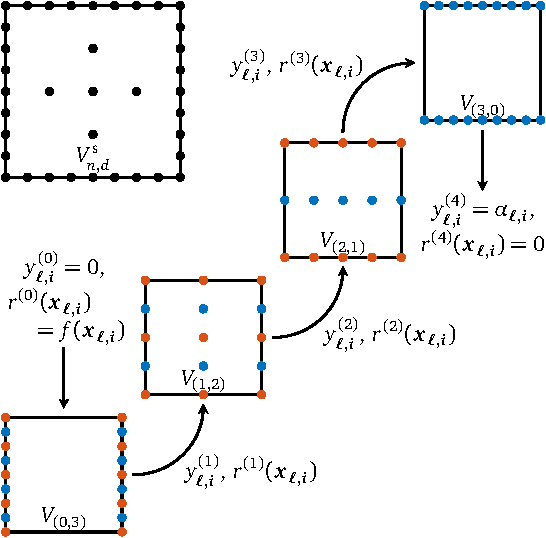
\includegraphics{residualInterpolation_1}%
  \caption[%
    Hierarchization with residual interpolation%
  ]{%
    Hierarchization of function value data on the
    two-dimensional regular sparse grid
    $\regsgspace{n}{d}$ of level $n = 3$ \emph{(top left)}
    using the method of residual interpolation.
    In this figure, we use
    $\linout[(j)]{\*l,\*i} \ceq \sum_{j'=1}^j \surplus[(j')]{\*l,\*i}$
    as an abbreviation.
    The order of the nodal spaces (here: bottom left to top right)
    does not matter.
    The data $\linout[(j)]{\*l,\*i}$
    corresponding to \textcolor{C0}{blue grid points}
    will not be modified in the remaining iterations
    and, therefore, already equals the correct surpluses $\surplus{\*l,\*i}$.
    The data corresponding to \textcolor{C1}{red grid points}
    will be modified as the grid points appear in one of the remaining
    nodal grids.%
  }%
  \label{fig:residualInterpolation}%
\end{SCfigure}
